% !TEX root = ../../main.tex
\section{Energy Based Methods}\label{sec:energy_based_methods}

Energy based methods have become very popular recently.

Given a graph $G = (U,V)$ we 
associate  a variable $ x_i \forall \quad u_i \in V$ with any node.
Within this thesis we focus on discrete energy function.
Therefore use discrete variables $x$.
W.l.o.g. we set  $ x_i   \in \{ 0,1,2,\ldots, N_{labels}-1 \} \quad \forall \quad u_i \in V$,
which means that any node has the same number of labels.

An energy function $E(x)$ can be  defined  in the following way:

\begin{equation} \label{eq:gm_energy}
E(x) = \sum_{v \in V} \phi_i(x_i) + \sum_{e=(i,j) \in E }\phi_{ij}(x_i,x_j) 
\end{equation}

Where the \emph{unaries} $\phi_i(x_i)$ encode local costs
for a variable to have certain label.
While the \emph{pairwise terms} $\phi_{ij}(x_i,x_j) $ define the interaction of adjacent nodes.
Often they are used to introduce some smoothness prior
into the model \citep{WHOM_TO_CITE_HERE} .


The vector which yields a minimum value of $E(x)$
is called $x_{\text{optimal}}$.

\begin{equation} \label{eq:gm_argmin}
x_{\text{optimal}} = \argmin_{x}  E(x)
\end{equation}


Before discussing how to optimize such an energy functions,
we will give some concrete examples how $E(X)$ 
can look in real world examples.

\paragraph{Denoising:}


Let $G=(V,E)$ be a grid graph corresponding to
a grayscale image.
Setting $N_{labels}$ to $255$ we can interpret  the variables $x$ directly as
gray values.
Let $I_i$ be the gray value of the pixel associated with variable $x_i$.

\begin{equation} \label{eq:gm_ef_dension}
E(x) = \sum_{v \in V}  (I_i - x_i)^2 + \sum_{e=(i,j) \in E } \lambda (x_i-x_j)^2
\end{equation}

\begin{figure}[H]
    \centering
    \subfloat[Input Image $I$]{ \label{fig:eq:gm_ef_dension_input}
        \includegraphics[width=0.25\textwidth]{fig/houseM-input.png}
    }
    \subfloat[ICM]{ \label{fig:eq:gm_ef_dension_icm}
        \includegraphics[width=0.25\textwidth]{fig/houseM-ICM.png}
    }
    \subfloat[$\alpha$-Expansion]{  \label{fig:eq:gm_ef_dension_ae}
        \includegraphics[width=0.25\textwidth]{fig/houseM-Expansion.png}
    }
    \subfloat[Trws]{  \label{fig:eq:gm_ef_dension_trws}
        \includegraphics[width=0.25\textwidth]{fig/houseM-TRW-S.png}
    }
    \caption[Energy based truncated denoising]{
        Finding $x_{\text{optimal}} $ for the energy function given
        in \cref{eq:gm_ef_dension} we show result of approximative solvers.
        Using \cref{fig:eq:gm_ef_dension_input} as input (for the black area no unaries 
        are used)
        the following
        results are obtained: ICM \cite{TODO_ICM}  (\Cref{fig:eq:gm_ef_dension_icm} ) fails
        to fill the in-painting area. While \cite{TODO_TRWS}  (\Cref{fig:eq:gm_ef_dension_trws} ) 
        and \cite{TODO_ALPHA_E}  (\Cref{fig:eq:gm_ef_dension_ae} ) can fill the in-painting area
        with meaningful values.
        The input image has been taken from \citep{szeliski_2008_pami}.
        The result images have been generated with OpenGM.
    }\label{fig:gm_ef_denoise}
\end{figure}

This model has been proposed by \citep{szeliski_2008_pami} where they proposed a MRF-benchmark.


\paragraph{Truncated Denoising:} 

This model is almost the same as the \emph{Denoising} model defined above,
but the second order term is truncate to $\gamma$ if $(x_i-x_j)^2$ is larger than $\gamma$.
Therefore we do pay only $\gamma$ at strong edges.
This model has also been proposed by \citep{szeliski_2008_pami} within their MRF-benchmark.


\begin{equation} \label{eq:gm_ef_dension_truncated}
E(x) = \sum_{v \in V}  (I_i - x_i)^2 + \sum_{e=(i,j) \in E } \lambda \cdot \min\left( (x_i-x_j)^2, \gamma\right)
\end{equation}

\begin{figure}[H]
    \centering
    \subfloat[Input Image $I$]{ \label{fig:eq:gm_ef_dension_truncated_input}
        \includegraphics[width=0.25\textwidth]{fig/penguin-bar.png}
    }
    \subfloat[ICM]{ \label{fig:eq:gm_ef_dension_truncated_icm}
        \includegraphics[width=0.25\textwidth]{fig/penguin-ICM.png}
    }
    \subfloat[$\alpha$-Expansion]{  \label{fig:eq:gm_ef_dension_truncated_ae}
        \includegraphics[width=0.25\textwidth]{fig/penguin-Expansion.png}
    }
    \subfloat[Trws]{  \label{fig:eq:gm_ef_dension_truncated_trws}
        \includegraphics[width=0.25\textwidth]{fig/penguin-TRW-S.png}
    }
    \caption[Energy based truncated denoising]{
        Finding $x_{\text{optimal}} $ for the energy function given
        in \cref{eq:gm_ef_dension_truncated} we show result of approximative solvers.
        Using \cref{fig:eq:gm_ef_dension_truncated_input} as input (for the black area no unaries 
        are used)
        the following
        results are obtained: ICM \cite{TODO_ICM}  (\Cref{fig:eq:gm_ef_dension_truncated_icm} ) fails
        to fill the in-painting area. While \cite{TODO_TRWS}  (\Cref{fig:eq:gm_ef_dension_truncated_trws} ) 
        and \cite{TODO_ALPHA_E}  (\Cref{fig:eq:gm_ef_dension_truncated_ae} ) can fill the in-painting area
        with meaningful values.
        The input image has been taken from \citep{szeliski_2008_pami}.
        The result images have been generated with OpenGM.
    }\label{fig:gm_ef_dension_truncated}
\end{figure}


\paragraph{Submodular Two Class Segmentation:}
    WRITE ME



\paragraph{Multicut Energy Function:}
Removing all unaries from \cref{eq:gm_energy} and 
setting $\phi_{ij}(x_i,x_j) =   \w_e \cdot \delta( x_i \neq x_j )$ 
will lead to the multicut objective (see \cref{sec:rw_multicut} and \cref{ch:cgc}) .

For planar problems  $N_{labels}$ can be set to 4 since any planar map is 4 colorable \citep{appel_1977_4color}.
For non planar problems we need to set $N_{labels}$ to $|V|$.



\begin{align}
E(x)=
    \sum_{ e=(i,j) \in E}
        \w_e \cdot \delta( x_i \neq x_j )
    \label{eq:gm_ef_multicut}
\end{align}


The \emph{max-cut} objective and  the multicut objective
are almost the same, 
but within max-cut problem we have only binary variable $x_i=\{0,1\}$ .

\begin{align}
E(x)=
    \sum_{ e=(i,j) \in E}
        \w_e \cdot \delta( x_i \neq x_j )
    \label{eq:gm_ef_max_cut}
\end{align}




\subsection{Graph Cut}

If $N_{labels}=2$ and $\phi_{ij}(x_i,x_j)$ is submodular, 
graph cuts \cite{GRAPH_CUT_INVENTOR} can be applied to find $x_{\text{optimal}}$
in polynomial time.

Graph cut is a optimization algorithm which reduces the energy minimizing problem
to the maximum flow / minimum cut problem. Energy function of binary variables which
have a form as 

\begin{equation}
\end{equation}




\begin{figure}[H]
\centering
\subfloat[$ $]{
    \includegraphics[height=0.3\textwidth]{fig/min_st.pdf}   
}
\hspace{1.5cm}
\subfloat[$ $]{
    \includegraphics[height=0.3\textwidth]{fig/min_st_d.pdf}   
}
\end{figure}


\subsection{QPBO}

\subsection{Multilabel Methods}

    cite all multilabel methods from opengm benchmark
